% Copyright (C) 2010,2011,2012,2013,2014,2015,2016 The ESPResSo project
% Copyright (C) 2002,2003,2004,2005,2006,2007,2008,2009,2010 
%   Max-Planck-Institute for Polymer Research, Theory Group
%  
% This file is part of ESPResSo.
%   
% ESPResSo is free software: you can redistribute it and/or modify it
% under the terms of the GNU General Public License as published by the
% Free Software Foundation, either version 3 of the License, or (at your
% option) any later version.
%  
% ESPResSo is distributed in the hope that it will be useful, but
% WITHOUT ANY WARRANTY; without even the implied warranty of
% MERCHANTABILITY or FITNESS FOR A PARTICULAR PURPOSE.  See the GNU
% General Public License for more details.
%  
% You should have received a copy of the GNU General Public License
% along with this program.  If not, see <http://www.gnu.org/licenses/>.
%
\documentclass[
a4paper,                        % paper size
11pt,                           % font size
twoside,                        % two sided
footsepline,                    % add a line to separate the footer
headsepline,                    % add a line to separate the header
headexclude,                    % header does not belong to the text
footexclude,                    % footer does not belong to the text
pagesize,                       % set the pagesize in a DVI document
]{scrartcl}

% Copyright (C) 2010,2011,2012 The ESPResSo project
% Copyright (C) 2002,2003,2004,2005,2006,2007,2008,2009,2010
%  Max-Planck-Institute for Polymer Research, Theory Group
%  
% This file is part of ESPResSo.
%   
% ESPResSo is free software: you can redistribute it and/or modify it
% under the terms of the GNU General Public License as published by the
% Free Software Foundation, either version 3 of the License, or (at your
% option) any later version.
%  
% ESPResSo is distributed in the hope that it will be useful, but
% WITHOUT ANY WARRANTY; without even the implied warranty of
% MERCHANTABILITY or FITNESS FOR A PARTICULAR PURPOSE.  See the GNU
% General Public License for more details.
%  
% You should have received a copy of the GNU General Public License
% along with this program.  If not, see <http://www.gnu.org/licenses/>.
%
\usepackage[draft]{varioref}    % defines \vref
\usepackage{hyperref}           % automatically creates links when
                                % using pdflatex, defines \url
\usepackage{ifpdf}              % defines \ifpdf
\usepackage{graphicx}           % handles graphics
\usepackage{color}              % use colors

\usepackage{amsmath}

\usepackage{verbatim}           % required for \verbatim and \endverbatim
\usepackage{fancyvrb}
\usepackage{calc}               % compute length
\usepackage{ifthen}             % provide ifthen
\usepackage{xspace}
\usepackage{units}
\usepackage[numbers]{natbib}

% For building the distribution docs, disable todo boxes.
%\usepackage[disable]{todonotes}
\usepackage{todonotes}

\newcommand{\es}{\mbox{\textsf{ESPResSo}}\xspace}
\newcommand{\ie}{\textit{i.e.}\xspace}
\newcommand{\eg}{\textit{e.g.}\xspace}
\newcommand{\etal}{\textit{et al.}\xspace}

\newcommand{\codebox}[1]%
{\texttt{#1}}

\DefineVerbatimEnvironment{code}{Verbatim}%
{commandchars=\\\{\}}
\makeatletter
\newenvironment{tclcode}
{%
  \addtolength{\linewidth}{-2em}% set the line length
  \@minipagetrue%%%DPC%%%
  \@tempswatrue%%%DPC%%%
  \hsize=\linewidth%
  \setbox0=\vbox\bgroup\verbatim
}{\endverbatim
  \unskip\setbox0=\lastbox%%%DPC%%%
  \egroup
  \par%
  \noindent\hspace{1em}%
  \codebox{\box0}%
  \par\noindent%
}
\makeatother

% \newcommand{\todo}[1]{
%   \marginpar{%
%     \setlength{\fboxrule}{1pt}
%     \fcolorbox{red}{yellow}{%
%       \parbox{\marginparwidth-2\fboxrule-2\fboxsep}{%
%         \bf\raggedright\scriptsize #1%
%       }%
%     }%
%   }%
% }

\makeatletter
\renewcommand{\minisec}[1]{\@afterindentfalse \vskip 1.5ex
  {\parindent \z@
    \raggedsection\normalfont\sffamily\itshape\nobreak#1\par\nobreak}%
  \@afterheading}
\makeatother

\newcommand{\esptitlehead}{
  \titlehead{
    \begin{center}
      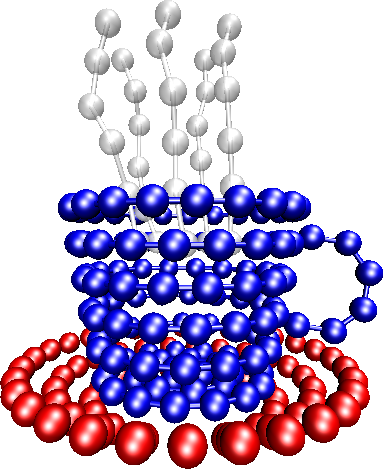
\includegraphics[width=5cm]{logo/transparentbg}
    \end{center}
  }
}


\begin{document}
\esptitlehead
\title{Tutorial 2: A simple charged system%
%\ifdefined\esversion%
%\thanks{For \es \esversion}%
%\fi%
}

\maketitle
\tableofcontents

\section{Introduction}

This tutorial introduces some of the basic features of \es\ for charged systems
by constructing a simulation script for a simple salt crystal. In the subsequent task,
we use to a more realistic force-field for a NaCl crystal. Finally, we introduce constraints
and 2D-Electrostatics to simulate a molten salt in a parallel plate capacitor.
We assume that the reader is familiar with the basic concepts of Python and MD simulations. The
code pieces can be copied step by step into a python script file, which then can
be run using \verb|pypresso <file>| from the \es build directory. Note that you might 
have to correct erroneous line breaks. Compile espresso with the following features 
in your \emph{myconfig.hpp} to be set throughout the whole tutorial:

\begin{pypresso}
#define EXTERNAL_FORCES
#define CONSTRAINTS
#define MASS
#define ELECTROSTATICS
#define LENNARD_JONES
\end{pypresso}

\section{Basic set up}

The script for the tutorial can be found in your build directory at\\
\verb|\doc\tutorials\python\02-charged_system\nacl.py|.
We start with importing numpy and the espressomd features and setting up all
the relevant simulation parameters in one place:

\begin{pypresso}

from espressomd import System, assert_features, electrostatics
import numpy

assert_features(["ELECTROSTATICS", "LENNARD_JONES"])


# System parameters
n_part = 200
n_ionpairs = n_part/2
density = 0.5
time_step = 0.01
temp = 1.0
gamma = 1.0
l_bjerrum = 7.0

num_steps_equilibration = 1000
num_configs = 100
integ_steps_per_config = 1000

# Particle parameters
types       = {"Anion":          0, "Cation": 1}
numbers     = {"Anion": n_ionpairs, "Cation": n_ionpairs}
charges     = {"Anion":       -1.0, "Cation": 1.0}
lj_sigmas   = {"Anion":        1.0, "Cation": 1.0}
lj_epsilons = {"Anion":        1.0, "Cation": 1.0}

WCA_cut = 2.**(1. / 6.)
lj_cuts     = {"Anion":  WCA_cut * lj_sigmas["Anion"], 
               "Cation": WCA_cut * lj_sigmas["Cation"]}
\end{pypresso}

These variables do not change anything in the simulation engine, but
are just standard Python variables. They are used to increase the
readability and flexibility of the script. The box length is not a
parameter of this simulation, it is calculated from the number of
particles and the system density. This allows to change the parameters
later easily, e.~g.\ to simulate a bigger system.
We use dictionaries for all particle related parameters, which is less error-prone and
readable as we will see later when we actually need the values. The parameters here define a purely repulsive, 
equally sized, monovalent salt.

The simulation engine itself is modified by changing the
espressomd.System() properties. We create an instance \pypressoinline{system} and
set the box length, periodicity and time step. The skin depth \pypressoinline{skin} 
is a parameter for the link--cell system which tunes its
performance, but shall not be discussed here. Further, we activate the Langevin thermostat
for our NVT ensemble with temperature \pypressoinline{temp} and friction coefficient \pypressoinline{gamma}. 


\begin{pypresso}
# Setup System
system = System()
box_l = (n_part / density)**(1. / 3.)
system.box_l = [box_l, box_l, box_l]
system.periodicity = [1, 1, 1]
system.time_step = time_step
system.cell_system.skin = 0.3
system.thermostat.set_langevin(kT=temp, gamma=gamma)
\end{pypresso}

We now fill this simulation box with particles at random positions, using type and charge from our dictionaries.
Using the length of the particle list \pypressoinline{system.part} for the id, we make sure that our particles are numbered consecutively.
The particle type is used to link non-bonded interactions to a certain group of particles.

\begin{pypresso}
# Place particles
for i in range(int(n_ionpairs)):
    system.part.add(
            id=len(system.part), 
            type=types["Anion"],  
            pos=numpy.random.random(3) * box_l, 
            q=charges["Anion"])
for i in range(int(n_ionpairs)):
    system.part.add(
            id=len(system.part), 
            type=types["Cation"], 
            pos=numpy.random.random(3) * box_l, 
            q=charges["Cation"])
\end{pypresso}

Before we can really start the simulation, we have to specify the
interactions between our particles. We already defined the Lennard-Jones parameters at the beginning,
what is left is to specify the combination rule and to iterate over particle type pairs. For simplicity, 
we implement only the \emph{Lorentz-Berthelot} rules. 
We pass our interaction pair to \pypressoinline{system.non_bonded_inter[*,*]} and set the 
pre-calculated LJ parameters \pypressoinline{epsilon}, \pypressoinline{sigma} and \pypressoinline{cutoff}. With \pypressoinline{shift="auto"},
we shift the interaction potential to the cutoff so that $U_{LJ}(r_{cutoff})=0$.

\begin{pypresso}
def combination_rule_epsilon(rule, eps1, eps2):
    if rule=="Lorentz":
        return (eps1*eps2)**0.5
    else:
        return ValueError("No combination rule defined")

def combination_rule_sigma(rule, sig1, sig2):
    if rule=="Berthelot":
        return (sig1+sig2)*0.5
    else:
        return ValueError("No combination rule defined")

# Lennard-Jones interactions parameters 
for s in [["Anion", "Cation"], 
          ["Anion", "Anion"], 
          ["Cation", "Cation"]]:
        lj_sig = combination_rule_sigma(
                "Berthelot",
                lj_sigmas[s[0]],lj_sigmas[s[1]])
        lj_cut = combination_rule_sigma(
                "Berthelot",
                lj_cuts[s[0]],lj_cuts[s[1]])
        lj_eps = combination_rule_epsilon(
                "Lorentz",
                lj_epsilons[s[0]],lj_epsilons[s[1]])

        system.non_bonded_inter[types[s[0]], types[s[1]]].lennard_jones.set_params(epsilon = lj_eps, sigma = lj_sig, cutoff = lj_cut, shift = "auto")

\end{pypresso}

\section{Equilibration}

With randomly positioned particles, we most likely have huge overlap and the strong repulsion will
cause the simulation to crash. The next step in our script therefore is a suitable LJ equilibration.
This is known to be a tricky part of a simulation and several approaches exist to reduce the particle overlap.
Here, we use a highly damped system (huge gamma in the thermostat) and cap the forces of the LJ interaction.
We use \pypressoinline{system.analysis.mindist} to get the minimal distance between all particles pairs. This value
is used to progressively increase the force capping. This results in a slow increase of the force capping at
strong overlap. At the end, we reset our thermostat to the target values and deactivate the force cap by setting 
it to zero.

\begin{pypresso}
print("\n--->Lennard Jones Equilibration")
max_sigma = max(lj_sigmas.values())
min_dist = 0.0
cap = 10.0
#Warmup Helper: Cold, highly damped system
system.thermostat.set_langevin(kT=temp*0.1, gamma=gamma*50.0)

while min_dist < max_sigma:
    #Warmup Helper: Cap max. force, increase slowly for overlapping particles
    min_dist = system.analysis.mindist(
            [types["Anion"],types["Cation"]],
            [types["Anion"],types["Cation"]])
    cap += min_dist
    system.force_cap = cap
    system.integrator.run(10)

#Don't forget to reset thermostat and force cap
system.thermostat.set_langevin(kT=temp, gamma=gamma)
system.force_cap = 0
\end{pypresso}

\es\ uses so-called \pypressoinline{actors} for electrostatics, magnetostatics and
hydrodynamics. This ensures that unphysical combinations of algorithms are
avoided, for example simultaneous usage of two electrostatic interactions.
Adding an actor to the system also activates the method and calls necessary
initialization routines. Here, we define a P$^3$M object with parameters Bjerrum
length and rms force error . This automatically starts a
tuning function which tries to find optimal parameters for P$^3$M and prints them
to the screen:

\begin{pypresso}
print("\n--->Tuning Electrostatics")
p3m = electrostatics.P3M(bjerrum_length=l_bjerrum, 
                         accuracy=1e-3)
system.actors.add(p3m)
\end{pypresso}

Before the production part of the simulation, we do a quick temperature 
equilibration. For the output, we gather all energies with
\pypressoinline{system.analysis.energy()}, calculate the "current" temperature\footnote{Note that for the ideal gas the temperature is given via $1/2 m \sqrt{\langle v^2 \rangle}=3/2 k_BT$, where $\langle \cdot \rangle$ denotes the ensemble average. Calculating some kind of "current temperature" via $T_\text{cur}=\frac{m}{3 k_B} \sqrt{ v^2 }$ you do not obtain the temperature in the system. Only when averaging the squared velocities first one would obtain the temperature for the ideal gas. $T$ is a fixed quantity and does not fluctuate in the canonical ensemble.} from the ideal part and 
print it to the screen along with the total and Coulomb energies.

We integrate for a certain amount of steps with \pypressoinline{system.integrator.run(100)}.

\begin{pypresso}
print("\n--->Temperature Equilibration")
system.time = 0.0
for i in range(int(num_steps_equilibration/100)):
    energy = system.analysis.energy()
    temp_measured = energy['kinetic'] / ((3.0 / 2.0) * n_part)
    print("t={0:.1f}, E_total={1:.2f}, E_coulomb={2:.2f}, 
          T={3:.4f}".format(system.time, energy['total'], 
          energy['coulomb'], temp_measured))
    system.integrator.run(100)
\end{pypresso}

\section{Running the simulation}

Now we can integrate the particle trajectories for a couple of time
steps. Our integration loop basically looks like the equilibration:

\begin{pypresso}
print("\n--->Integration")
system.time = 0.0
for i in range(num_configs):
    energy = system.analysis.energy()
    temp_measured = energy['kinetic'] / ((3.0 / 2.0) * n_part)
    print("t={0:.1f}, E_total={1:.2f}, E_coulomb={2:.2f},
            T={3:.4f}".format(system.time, energy['total'],
            energy['coulomb'], temp_measured))
    system.integrator.run(integ_steps_per_config)

    # Internally append particle configuration
    system.analysis.append()
\end{pypresso}

Additionally, we append all particle configurations in the core with \pypressoinline{system.analysis.append()} for
a very convenient analysis later on. 

\begin{figure}[tb]
  \centering
  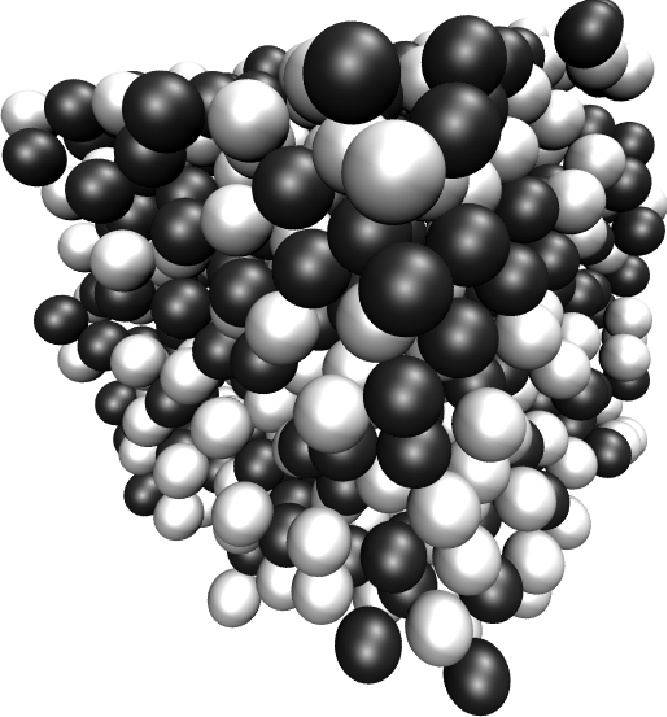
\includegraphics[width=0.3\textwidth]{figures/salt}
  \caption{VMD Snapshot of the salt system}
  \label{fig:snapshot}
\end{figure}

\section{Analysis}

Now, we want to calculate the averaged radial distribution functions
$g_{++}(r)$ and $g_{+-}(r)$ with the \pypressoinline{rdf()} command from \pypressoinline{system.analysis}: 

\begin{pypresso}
print("\n--->Analysis")
# Calculate the averaged rdfs
rdf_bins = 100
r_min  = 0.0
r_max  = system.box_l[0]/2.0
r,rdf_00 = system.analysis.rdf(rdf_type='<rdf>', 
                            type_list_a=[types["Anion"]],
                            type_list_b=[types["Anion"]], 
                            r_min=r_min,
                            r_max=r_max, 
                            r_bins=rdf_bins)
r,rdf_01 = system.analysis.rdf(rdf_type='<rdf>',
                            type_list_a=[types["Anion"]],
                            type_list_b=[types["Cation"]], 
                            r_min=r_min, r_max=r_max, r_bins=rdf_bins)

\end{pypresso}

The shown \pypressoinline{rdf()} commands return the radial distribution functions for
equally and oppositely charged particles for specified radii and number of bins. 
In this case, we calculate the averaged rdf of the stored
configurations, denoted by the chevrons in \pypressoinline{rdf_type='<rdf>'}. Using
\pypressoinline{rdf_type='rdf'} would simply calculate the rdf of the current particle
configuration. The results are two NumPy arrays containing the $r$ and $g(r)$
values. Finally we write the data into a file with standard python output routines.

\begin{pypresso}
with open('rdf.data', 'w') as rdf_fp:
    for i in range(rdf_bins):
        rdf_fp.write("%1.5e %1.5e %1.5e\n" % 
                (r[i], rdf_00[i], rdf_01[i]))
print("\n--->Written rdf.data\n--->Done")
\end{pypresso}

\begin{figure}[tb]
  \centering
  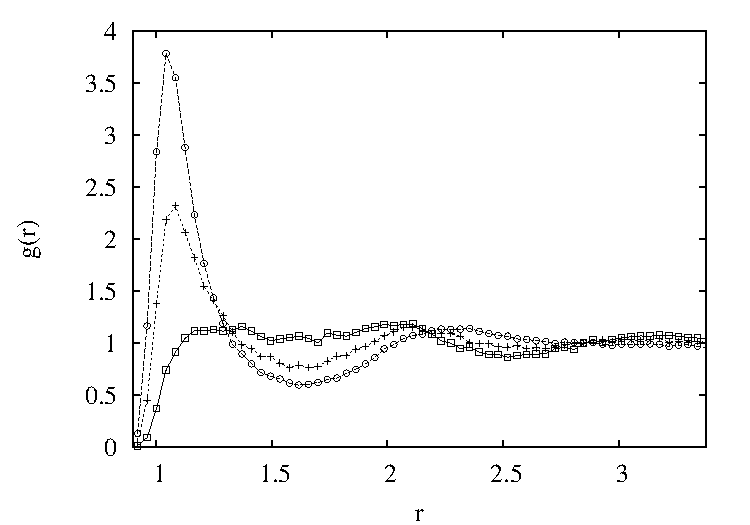
\includegraphics[width=0.6\textwidth]{figures/nacl-rdf}
  \caption{Radial distribution functions $g_{++}(r)$ between equal
    charges (rectangles) and $g_{+-}(r)$ for opposite charges
    (circles). The plus symbols denote $g(r)$ for an uncharged
    system.}
  \label{fig:rdf}
\end{figure}

Fig.~\ref{fig:rdf} shows the resulting radial distribution functions. In
addition, the distribution for a neutral system is given, which can be obtained
from our simulation script by simply not adding the P$^3$M actor to the system.
To view your own results, run \pypressoinline{gnuplot} in a Terminal window
and plot the simulation data:

\begin{pypresso}
p 'rdf.data' u 1:2 w lp t 'g(r) ++' , '' u 1:3 w lp t 'g(r) +-'
\end{pypresso}

\section{Task - Real units}

So far, the system has arbitrary units and is not connected to any real physical system.
Simulate a proper NaCl crystal with the force field parameter taken from:\\
\\
\noindent R. Fuentes-Azcatl and M. Barbosa, \emph{Sodium Chloride, NaCl/$\epsilon$ : New Force Field},\\ J. Phys. Chem. B, 2016, 120(9), pp 2460-2470
\begin{table}[h]
    \centering
    \begin{tabular}{l|llll}
           & $q/\mathrm{e}$  & $\sigma / \mathrm{\AA} $ & $(\epsilon /\mathrm{k_B})/\mathrm{K}$ & $m/\mathrm{u}$  \\
        \hline
        Na & +1     & 2.52          & 17.44                 & 22.99  \\
        \hline
        Cl & -1     & 3.85          & 192.45                & 35.453 
    \end{tabular}
\end{table}

Use the following system parameters:

\begin{table}[h]
    \centering
    \begin{tabular}{l|l}
        Temperature            & $298 \ \mathrm{K}$          \\
        \hline
        Friction Coeff.        & $10 \ \mathrm{ps^{-1}}$      \\
        \hline
        Density                & $1.5736 \ \mathrm{u \AA^{-3}}$ \\
        \hline
        Bjerrum length($298 \ \mathrm{K}$) & $439.2 \ \mathrm{\AA}$      \\
        \hline
        Time step              & $2 \ \mathrm{fs}$
    \end{tabular}
\end{table}

To make your life more easy, don't try to equilibrate randomly positioned particles,
but set them up in a crystal structure close to equilibrium. If you do it right,
you don't even need the Lennard-Jones equilibration. 
To speed things up, don't go further than 1000 particles and use a P$^3$M accuracy of $10^{-2}$.
Your RDF should look like the plot in figure \ref{fig:nacl_units}. When you get stuck,
you can look at the solution script \verb|\doc\tutorials\python\02-charged_system\nacl_units.py| 
(or \verb|nacl_units_vis.py| with visualization).


\begin{figure}[h]
  \centering
  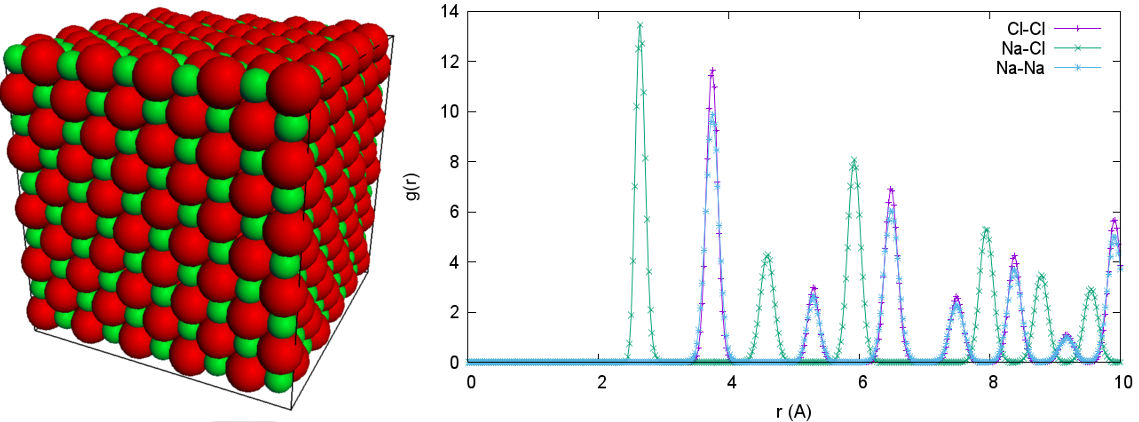
\includegraphics[width=0.9\textwidth]{figures/nacl_units}
  \caption{Snapshot and RDF of the parametrized NaCl crystal.}
  \label{fig:nacl_units}
\end{figure}

\section{2D Electrostatics and Constraints}

In this section, we use the parametrized NaCl system from the last task to simulate a molten salt in a
parallel plate capacitor with and without applied electric field. We have to extend our simulation by several aspects:

\paragraph{Confinement}\mbox{}\\
\es features a number of basic shapes like cylinders, walls or spheres to simulate confined systems.
Here, we use to walls at $z = 0$ and $z = L_z$ for the parallel plate setup ($L_z$: Box length in z-direction).
\paragraph{2D-Electrostatics}\mbox{}\\
\es also has a number of ways to account for the unwanted electrostatic interaction in the now non-periodic z-dimension.
We use the 3D-periodic P$^3$M algorithm in combination with the \emph{Electrostatic Layer Correction} (ELC). 
ELC subtracts the forces caused by the periodic images in the z-dimension. Another way would be to use the explicit 2D-electrostatics algorithm
MMM2D, also available in \es.
\paragraph{Electric Field}\mbox{}\\
The simple geometry of the system allows us to treat an electric field in z-direction as a homogeneous force.
Note that we use inert walls here and don't take into account the dielectric contrast caused by metal electrodes.
\paragraph{Parameters}\mbox{}\\
For our molten NaCl, we use a temperature $100 \ \mathrm{K}$ above the melting point ($1198.3 \ \mathrm{K}$) 
and an approximated density of $\rho = 1.1138 \ \mathrm{u \AA^{-3}}$ found in \\
Janz, G. J., Thermodynamic and Transport Properties of Molten Salts: Correlation Equations for Critically Evaluated Density, Surface Tension,
Electrical Conductance, and Viscosity Data, \emph{J. Phys. Chem. Ref. Data, 17}, Suppl. 2, 1988.\\

Let's walk through the python script. We need additional imports for the wall shapes and the ELC algorithm:

\begin{pypresso}
from espressomd import System, assert_features, electrostatics, electrostatic_extensions, shapes
import numpy
\end{pypresso}

If we target a liquid system, we should not set up the particles in a lattice, 
as this introduces unwanted structure in the starting configuration.
We define our system size by the number of particles and the density.
The system parameters lead to the following values:

\begin{pypresso}
system = System()

print("\n--->Setup system")

# System parameters
n_part = 500
n_ionpairs = n_part/2
density = 1.1138
time_step = 0.001823
temp = 1198.3
gamma = 50
#l_bjerrum = 0.885^2 * e^2/(4*pi*epsilon_0*k_B*T)
l_bjerrum = 130878.0 / temp
wall_margin = 0.5
Ez = 0

num_steps_equilibration = 3000
num_configs = 200
integ_steps_per_config = 100
\end{pypresso}

We save the force field parameters in python dictionaries, now with parameters for the walls:

\begin{pypresso}
# Particle parameters
types       = {"Cl":          0, "Na": 1, "Electrode": 2}
numbers     = {"Cl": n_ionpairs, "Na": n_ionpairs}
charges     = {"Cl":       -1.0, "Na": 1.0}
lj_sigmas   = {"Cl":       3.85, "Na": 2.52,  "Electrode": 3.37}
lj_epsilons = {"Cl":     192.45, "Na": 17.44, "Electrode": 24.72}

lj_cuts     = {"Cl":        3.0 * lj_sigmas["Cl"], 
               "Na":        3.0 * lj_sigmas["Na"],
               "Electrode": 3.0 * lj_sigmas["Electrode"]}

masses      = {"Cl":  35.453, "Na": 22.99, "Electrode": 12.01}
\end{pypresso}

To finally calculate the box size, we take into account the diameter of the electrode interaction.
Additionally, ELC needs a particle-free gap in the z-direction behind the wall.

\begin{pypresso}
# Setup System
box_l = (n_ionpairs * sum(masses.values()) / density)**(1. / 3.)
box_z = box_l + 2.0 * (lj_sigmas["Electrode"]+wall_margin)
box_volume = box_l * box_l * box_z
elc_gap = box_z * 0.15
system.box_l = [box_l, box_l, box_z + elc_gap]
system.periodicity = [1, 1, 1]
system.time_step = time_step
system.cell_system.skin = 0.3
system.thermostat.set_langevin(kT=temp, gamma=gamma)
\end{pypresso}

In the next snippet, we add the walls to our system. Our constraint takes two arguments: 
First the \pypressoinline{shape}, in our case a simple plane defined by its normal vector and the distance from the origin, 
second the \pypressoinline{particle_type}, which is used to set up the interaction between particles and constraints.

\begin{pypresso}
# Walls   
system.constraints.add(shape=Wall(dist=wall_margin,
            normal=[0,0,1]),particle_type=types["Electrode"])
system.constraints.add(shape=Wall(dist=-(box_z-wall_margin),
            normal=[0,0,-1]),particle_type=types["Electrode"])
\end{pypresso}

Now we place the particles at random position without overlap with the walls:

\begin{pypresso}
# Place particles
for i in range(int(n_ionpairs)):
    p = numpy.random.random(3)*box_l
    p[2] += lj_sigmas["Electrode"]
    system.part.add(id=len(system.part), type=types["Cl"],  pos=p, q=charges["Cl"], mass=masses["Cl"])
for i in range(int(n_ionpairs)):
    p = numpy.random.random(3)*box_l
    p[2] += lj_sigmas["Electrode"]
    system.part.add(id=len(system.part), type=types["Na"],  pos=p, q=charges["Na"], mass=masses["Na"])
\end{pypresso}

The scheme to set up the Lennard-Jones interaction is the same as before, 
extended by the Electrode-Ion interactions:

\begin{pypresso}
# Lennard-Jones interactions parameters 

def combination_rule_epsilon(rule, eps1, eps2):
    if rule=="Lorentz":
        return (eps1*eps2)**0.5
    else:
        return ValueError("No combination rule defined")

def combination_rule_sigma(rule, sig1, sig2):
    if rule=="Berthelot":
        return (sig1+sig2)*0.5
    else:
        return ValueError("No combination rule defined")

for s in [["Cl", "Na"], ["Cl", "Cl"], ["Na", "Na"], ["Na", "Electrode"], ["Cl", "Electrode"]]:
        lj_sig = combination_rule_sigma("Berthelot", 
                lj_sigmas[s[0]], lj_sigmas[s[1]])
        lj_cut = combination_rule_sigma("Berthelot", 
                lj_cuts[s[0]], lj_cuts[s[1]])
        lj_eps = combination_rule_epsilon("Lorentz", 
                lj_epsilons[s[0]],lj_epsilons[s[1]])

        system.non_bonded_inter[types[s[0]], types[s[1]]].
            lennard_jones.set_params(epsilon=lj_eps, 
            sigma=lj_sig, cutoff=lj_cut, shift="auto")
\end{pypresso}

Next is the Lennard-Jones Equilibration. Here we use an alternative way to get rid of the overlap: \es features a routine for energy
minimization with similar features as in the manual implementation used before. Basically it 
caps the forces and limits the displacement during integration.

\begin{pypresso}
energy = system.analysis.energy()
print("Before Minimization: E_total=", energy['total'])
system.minimize_energy.init(f_max = 10, gamma = 10.0, 
        max_steps = 1000, max_displacement= 0.2)
system.minimize_energy.minimize()
energy = system.analysis.energy()
print("After Minimization: E_total=", energy['total'])
\end{pypresso}

As described, we use P$^3$M in combination with ELC to account for the 2D-periodicity. 
ELC is also added to the \pypressoinline{actors} of the system and takes \emph{gap size} and \emph{maximum
pairwise errors} as arguments.

\begin{pypresso}
print("\n--->Tuning Electrostatics")
p3m = electrostatics.P3M(bjerrum_length=l_bjerrum, 
        accuracy=1e-2)
system.actors.add(p3m)
elc = electrostatic_extensions.ELC(gap_size = elc_gap, 
        maxPWerror = 1e-3)
system.actors.add(elc)
\end{pypresso}

For now, our electric field is zero, but we want to switch it on later.
Here we run over all particles and set an external force on the charges caused 
by the field:

\begin{pypresso}
for p in system.part:
    p.ext_force = [0,0,Ez * p.q]
\end{pypresso}

This is followed by our standard temperature equilibration:

\begin{pypresso}
print("\n--->Temperature Equilibration")
system.time = 0.0
for i in range(int(num_steps_equilibration/100)):
    energy = system.analysis.energy()
    temp_measured = energy['kinetic'] / ((3.0 / 2.0) * n_part)
    print("t={0:.1f}, E_total={1:.2f}, E_coulomb={2:.2f},
          T={3:.4f}".format(system.time, energy['total'],
          energy['coulomb'], temp_measured))
    system.integrator.run(100)
\end{pypresso}

In the integration loop, we like to measure the density profile for both ion species along the z-direction.
We use a simple histogram analysis to accumulate the density data.

\begin{pypresso}
print("\n--->Integration")
bins=100
z_dens_na = numpy.zeros(bins)
z_dens_cl = numpy.zeros(bins)
system.time = 0.0
cnt = 0

for i in range(num_configs):
    energy = system.analysis.energy()
    temp_measured = energy['kinetic'] / ((3.0 / 2.0) * n_part)
    print("t={0:.1f}, E_total={1:.2f}, E_coulomb={2:.2f},
          T={3:.4f}".format(system.time, energy['total'],
          energy['coulomb'], temp_measured))
    system.integrator.run(integ_steps_per_config)

    for p in system.part:
        bz = int(p.pos[2]/box_z*bins)
        if p.type == types["Na"]:
            z_dens_na[bz] += 1.0
        elif p.type == types["Cl"]:
            z_dens_cl[bz] += 1.0
    cnt += 1
\end{pypresso}

Finally, we calculate the average, normalize the data with the bin volume and save it to
a file using NumPy's \pypressoinline{savetxt} command.

\begin{pypresso}
print("\n--->Analysis")
#Average / Normalize with Volume
z_dens_na /= (cnt * box_volume/bins)
z_dens_cl /= (cnt * box_volume/bins)
z_values = numpy.linspace(0,box_l,num=bins)
res = numpy.column_stack((z_values,z_dens_na,z_dens_cl))
numpy.savetxt("z_density.data",res,
        header="#z rho_na(z) rho_cl(z)")
print("\n--->Written z_density.data")
print("\n--->Done")
\end{pypresso}

The resulting density plot is very noisy due to insufficient sampling, but should show a slight depletion of the smaller Na atoms
at the walls. Now try to put in an electric field that represents an applied voltage of $15 \ \mathrm{V}$ between the walls and compare the results.
The density data (see figure \ref{fig:nacl_confined}) should show strong layering at the walls, decaying towards the system center.
The complete script is at \\
\verb|\doc\tutorials\python\02-charged_system\nacl_units_confined.py|.\\
In the interactive script \verb|nacl_units_confined_vis.py|, you can increase/decrease the electric field with the keys \emph{u/j} (at your own risk).

\begin{figure}[tb]
  \centering
  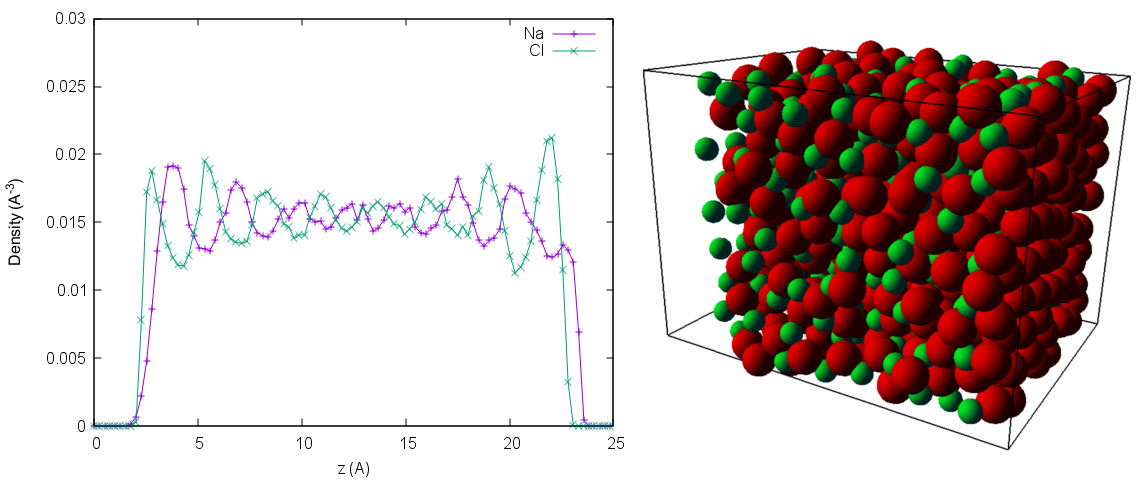
\includegraphics[width=0.9\textwidth]{figures/nacl_units_confined}
  \caption{Snapshot and densities along the z-Axis with applied electric field for the ion species.}
  \label{fig:nacl_confined}
\end{figure}

\end{document}
